% ****** Start of file apssamp.tex ******
%
%   This file is part of the APS files in the REVTeX 4.1 distribution.
%   Version 4.1r of REVTeX, August 2010
%
%   Copyright (c) 2009, 2010 The American Physical Society.
%
%   See the REVTeX 4 README file for restrictions and more information.
%
% TeX'ing this file requires that you have AMS-LaTeX 2.0 installed
% as well as the rest of the prerequisites for REVTeX 4.1
%
% See the REVTeX 4 README file
% It also requires running BibTeX. The commands are as follows:
%
%  1)  latex apssamp.tex
%  2)  bibtex apssamp
%  3)  latex apssamp.tex
%  4)  latex apssamp.tex
%
\documentclass[%
 reprint,
%superscriptaddress,
%groupedaddress,
%unsortedaddress,
%runinaddress,
%frontmatterverbose, 
%preprint,
%showpacs,preprintnumbers,
%nofootinbib,
%nobibnotes,
%bibnotes,
 amsmath,amssymb,
 aps,
%pra,
%prb,
%rmp,
%prstab,
%prstper,
%floatfix,
]{revtex4-1}

\usepackage{graphicx}% Include figure files
\usepackage{dcolumn}% Align table columns on decimal point
\usepackage{bm}% bold math
%\usepackage{hyperref}% add hypertext capabilities
%\usepackage[mathlines]{lineno}% Enable numbering of text and display math
%\linenumbers\relax % Commence numbering lines

%\usepackage[showframe,%Uncomment any one of the following lines to test 
%%scale=0.7, marginratio={1:1, 2:3}, ignoreall,% default settings
%%text={7in,10in},centering,
%%margin=1.5in,
%%total={6.5in,8.75in}, top=1.2in, left=0.9in, includefoot,
%%height=10in,a5paper,hmargin={3cm,0.8in},
%]{geometry}

\begin{document}

%\preprint{APS/123-QED}

\title{Filtering twitter feed}% Force line breaks with \\
% \thanks{A footnote to the article title}%

\author{Alexey Levin}
%  \email{lvn@bu.edu}
%  \altaffiliation[Also at ]{Physics Department, Boston University.}%Lines break automatically or can be forced with \\
\author{Aaron Elliot}%
%  \email{aelliot@institution.edu}
\affiliation{%
 Boston University
}%

% \collaboration{MUSO Collaboration}%\noaffiliation

% \author{Charlie Author}
%  \homepage{http://www.Second.institution.edu/~Charlie.Author}
% \affiliation{
%  Second institution and/or address\\
%  This line break forced% with \\
% }%
% \affiliation{
%  Third institution, the second for Charlie Author
% }%
% \author{Delta Author}
% \affiliation{%
%  Authors' institution and/or address\\
%  This line break forced with \textbackslash\textbackslash
% }%

% \collaboration{CLEO Collaboration}%\noaffiliation

\date{\today}% It is always \today, today,
             %  but any date may be explicitly specified

\begin{abstract}


We consider data from twitter, working with text contents of tweets.
Our purpose is to obtain classification of tweets, which could be applied to user's feed to filter it.
The classification is done using LSA and applying GMM or Kmeans afterwards.
% We show that resulting clusters are ... (!!!)
We also build network of user interactions, using mentions in tweets. Network structure then can be used to complement the classifier and improve relevance of a particular users' feed.

% ful in determining tweets that are relevant to the user, but posted from outside of the set of people they follow.


% \begin{description}
% \item[Usage]
% Secondary publications and information retrieval purposes.
% \item[PACS numbers]
% May be entered using the \verb+\pacs{#1}+ command.
% \item[Structure]
% You may use the \texttt{description} environment to structure your abstract;
% use the optional argument of the \verb+\item+ command to give the category of each item. 
% \end{description}
\end{abstract}



% \pacs{Valid PACS appear here}% PACS, the Physics and Astronomy
                             % Classification Scheme.
%\keywords{Suggested keywords}%Use showkeys class option if keyword
                              %display desired
\maketitle

%\tableofcontents

\section{\label{sec:level1}Problem}

% Intro, Problem.

Twitter is one of the most heavily used services today. 
It is a social media platform that lets users publish their thoughts in form of short 'tweets' - posts that are at most 140 characters long.
The brief nature of communications on twitter make it a very 'real-time' platform, where large volumes of posts can appear in a very short time.

This poses a problem: a particular user's feed (tweets from everyone they are subscribed to) becomes extremely cluttered, to the extent of being useless. Also, different accounts post with frequencies varying by many orders of magnitude, so feed becomes dominated by most abundant, noisy channels, which makes the average importance of tweets in the feed low.



\section{Method}

Ultimately the solution is to offer some filtering method.

The methods that could be used to approach this problem could be:
\begin{itemize}
    \item[a)] Ranking tweets by 'importance' or 'relevance'. \\
    % \textit{Downside: highly subjective.}
    Downside: highly subjective.

    \item[b)] Classifying tweets into categories.\\
    %!!!
	Downside: does not ultimately tune to user, user still has work to do, by choosing which categories to read. 
	However, categories could be determined based on "importance" of information (as in 'casual chat' vs 'breaking news'), which solves original problem.
% 	there is hope that categories might look as 'meaningful', 'trash', containing 'importance' information in them too 
\end{itemize}

The problem with a) is that it highly depends on user, so needs a lot of complementary information (user features, ground truth labeling for each user).

Our strategy is to use b) to classify tweets. After that the filtering can be done by choosing particular slices from feed (eg. "updates from friends + politics").

We also analyze the network structure of user relations on twitter, where an edge connects users if one of them has mentioned the other in a tweet. That can be helpful in determining tweets from which users are relevant to a particular one.

We base our analysis solely on text data from tweets (ignoring metadata), because in this case the approach can be easily reapplied to any other blogging platform (facebook feed, etc).



\section{Obtaining data}
%!!! replace https with articles
We wrote a parser that accesses tweets from twitter API.
We also found several academic datasets \cite{sentiment140, sanalyt} that are suitable for our task, which we used to enlarge the size of dataset we are working with.
We were able to access the whole tweet object through API.
The datasets contain very limited information about tweets, however it is more than enough for our purposes, because we are only interested in the text contents of tweets themselves.
We merged data from all of these sources and used that as our dataset.



\section{Data preparation}

Our analysis consisted of two components: analysis of network structure and NLP.

First thing we had to do was construct the network. We did this by parsing texts of tweets using regular expressions and adding an edge between users if one of them mentions the other.

For the document-term analysis, we used 'bag of words' approach and TfIdf technique to vectorize the data (using english stopwords dictionary and thresholding the term frequency on both sides to clean data of corpus specific stopwords or irrelevant terms that appear only in a few documents). Finally, we reduced the dimensionality of our data by performing PCA. We keep 15 largest singular values in our further analysis.


\section{Analysis}

\subsection{Basic properties of data.}

Our final dataset had approximately 1610000 tweets from 660000 users. The network of mentions, which also contains users from outside of dataset that were mentioned had approximately 900000 nodes and 620000 edges. The largest connected component that we are working with has $\sim 340000$ nodes.

% The basic properties of the data we had were:
% ...


\subsection{Network}

For the network data we efficiently found clusters (communities) using Kmeans++ on spectral representation of a network using 5 lowest non-zero eigenvectors.

\begin{figure}[htp]
\centering
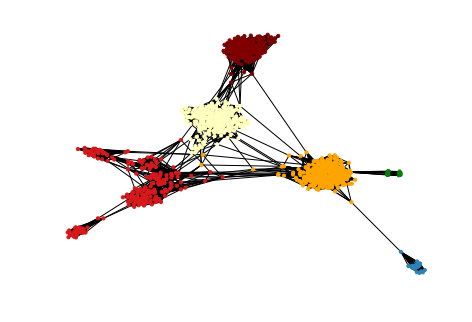
\includegraphics[width=10cm]{communities}
\caption{Communities in the network of mentions on twitter, using spectral decomposition and kmeans++.}
\label{fig}
\end{figure}
%!!! weird figs...

% \begin{figure}[htp]
% \centering
% 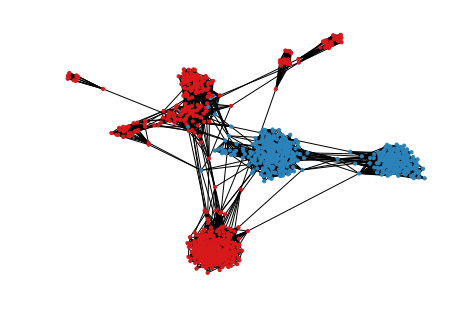
\includegraphics[width=10cm]{fiedler}
% \caption{Cutting the graph using Fiedler vector.}
% \label{fig}
% \end{figure}

We performed basic analysis of the network that we built out of user mentions. Indeed, the network exhibits all the expected properties of a real world-network. In particular, degrees are distributed as a power law.

\begin{figure}[htp]
\centering
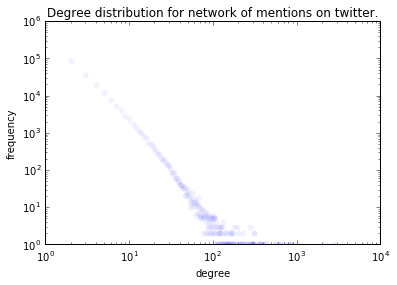
\includegraphics[width=9cm]{deg_dist}
\caption{Degree distribution.}
\label{fig}
\end{figure}

% Core size distribution.

Properties of relations between users in the network of mentions give methods of predicting relevance of a tweet to the user (using network-based similarity measures) that are complementary to the NLP analysis.


\newpage

\subsection{NLP.}

We used clustering with Gaussian Mixture Models and Kmeans++ to find topics that people talk about.

We analyzed the terms that were most popular in each cluster.

Almost every cluster had as it's most popular terms words related to time, especially to currents moment (such as \textit{now, today, tomorrow, morning} and such), and words related to \textit{work} or \textit{school}.

The most obvious differentiator between clusters was, maybe surprisingly, the sentiment. The most defined discrepancies between clusters would be the proliferation of terms such as \textit{sad, sick, tired, need}, or \textit{happy, awesome, sunny, weekend}. The topics are not distinctly separated. We conclude that standard methods for clustering rather detect the mood of tweets, than the topic. Also we found that, as expected, twitter is mainly used to express emotions or feelings related to what is happening at the moment. 
% However, we could still arguably detect some categories that help solve the original problem of classification. 

\begin{figure}[htp]
\centering
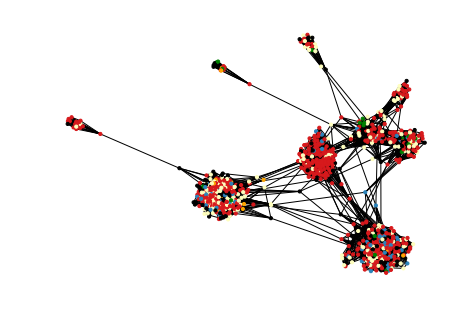
\includegraphics[width=9cm]{lsa_on_graph}
\caption{The nodes are colored according to LSA clustering. Popular topics are not driven by belonging to a particular community.}
\label{fig}
\end{figure}


Comparing clusters to network data we observe the following.
Mentioning communities on twitter are not interest-based. 
The distribution of topics that people tweet about is homogeneous over the network. So, communities are rather 'College 1', 'College 2', than 'divers', 'football players', and the topics spoken about in College 1 and College 2 are same.










\bibliographystyle{unsrt}
\bibliography{ref}

\end{document}